\chapter{Ironic简介}
Ironic是OpenStack社区用于管理裸机(物理机)的一个项目。

\section{适用场景}

针对高性能,cpu密集型计算服务,原有的虚拟机在很多场景下已经不再适用,尤其是虚拟
机的性能受到qemu以及物理机硬件本身虚拟化的各种限制,无法提供更高的计算性能。Ironic
项目的目的就是为了解决这些问题。
\par Ironic最适用的场景:
\begin{itemize}
  \item 高性能计算集群
  \item 物理硬件无法被虚拟化
  \item 数据库集群,特别是oracle的数据库集群
\end{itemize}

\section{逻辑架构}

图 \nameref{fig:logical_architecture}
直观的描述了Ironic的几个重要的概念以及组成部分

\begin{enumerate}
  \item Ironic API:提供API访问接口,供外部调用
  \item Ironic Conductor:真实的工作流程的处理。处理API提交过来的任务。API和Conductor之间通过RPC通信
  \item Driver:真正处理Ironic具体业务的驱动程序。一般是PXE或者IMPL之类的硬件管理模块
  \item 消息队列:传递相关的消息
  \item 数据库:保存Ironic的重要数据
\end{enumerate}

% H 表示图表的位置保持不变,不再是浮动体
% H选项与thbp不兼容
\begin{figure}[H]
  \centering
  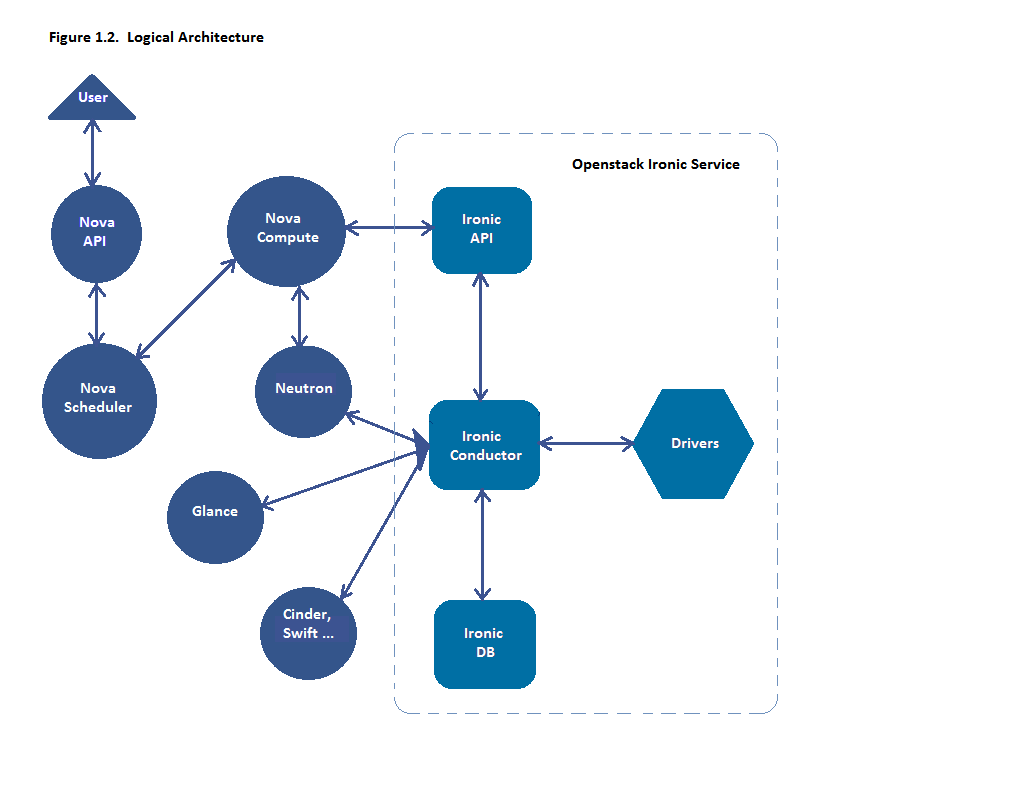
\includegraphics[scale=0.8]{logical_architecture.png}
  \caption{Ironic逻辑架构图\protect\footnotemark}
  \label{fig:logical_architecture}
\end{figure}
\footnotetext{来源:\url{http://docs.openstack.org/developer/ironic/_images/logical_architecture.png}}
% 在caption当中不能直接使用footnote,而需要\protect\footnotemark与\footnotetext
% 共同使用

\section{关键技术}
由于Ironic管理的是物理服务器,因此,需要用到以下的几种技术来支持。同样的,如果
需要将物理服务器纳入Ironic的管理,也需要这些技术的支持。

\begin{itemize}
  \item PXE
  \item DHCP
  \item NBP
  \item TFTP
  \item IPMI
\end{itemize}

\section{部署架构}

\begin{figure}[H]
  \centering
  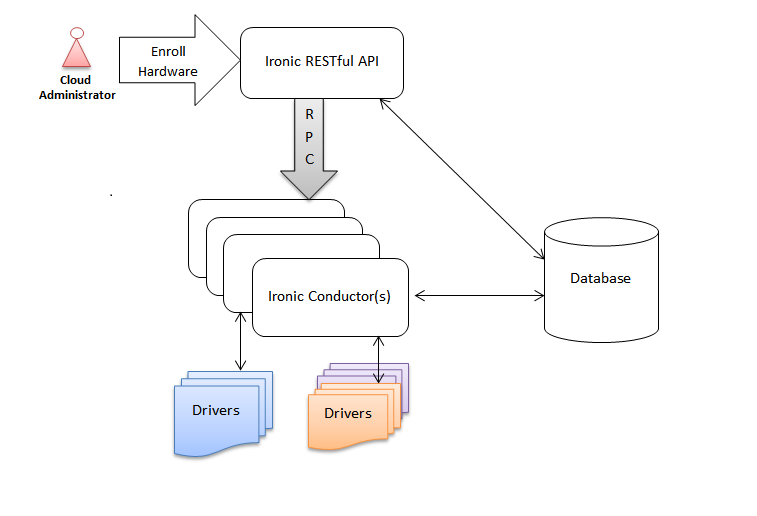
\includegraphics[scale=0.8]{deployment_architecture.png}
  \caption{Ironic部署架构图\protect\footnotemark}
  \label{fig:deployment_architecture}
\end{figure}
\footnotetext{来源:\url{http://docs.openstack.org/developer/ironic/_images/deployment_architecture_2.png}}

实际生产时,一个Ironic集群可以有多个API服务(需要使用负载均衡软件负载),有多个
Conductor。每个Conductor可以对接多个不同的Driver。Conductor是多活,并且是高度可用的。
Ironic在设计时就考虑了整个架构的高可用和高稳定性。

\section{理解裸机部署}
Ironic本身是被设计用于物理主机的部署。在使用Ironic部署物理服务器时,它的内部机制
是如何进行的,我们可以探讨一下。
\par 但在探讨部署物理机之前,需要满足以下条件:
\begin{itemize}
  \item Ironic服务已经被正确部署,并且没有任何错误。同时,Ironic所依赖的第三方服务也运行正常,包括tftp,impi等等。
  \item Nova的compute driver必须配置为Ironic,而不再是虚拟化的driver。
  \item Flavor必须根据具体的硬件配置进行调整
  \item Glance存在可用的Image镜像文件。支持的镜像格式如下:
  \begin{itemize}
    \item bm-deploy-kernel
    \item bm-deploy-ramdisk
    \item user-image
    \item user-image-vmlinuz
    \item user-image-initrd
  \end{itemize}
  \item 物理主机已经提前加入Ironic的管理范围
\end{itemize}

\begin{figure}[H]
  \centering
  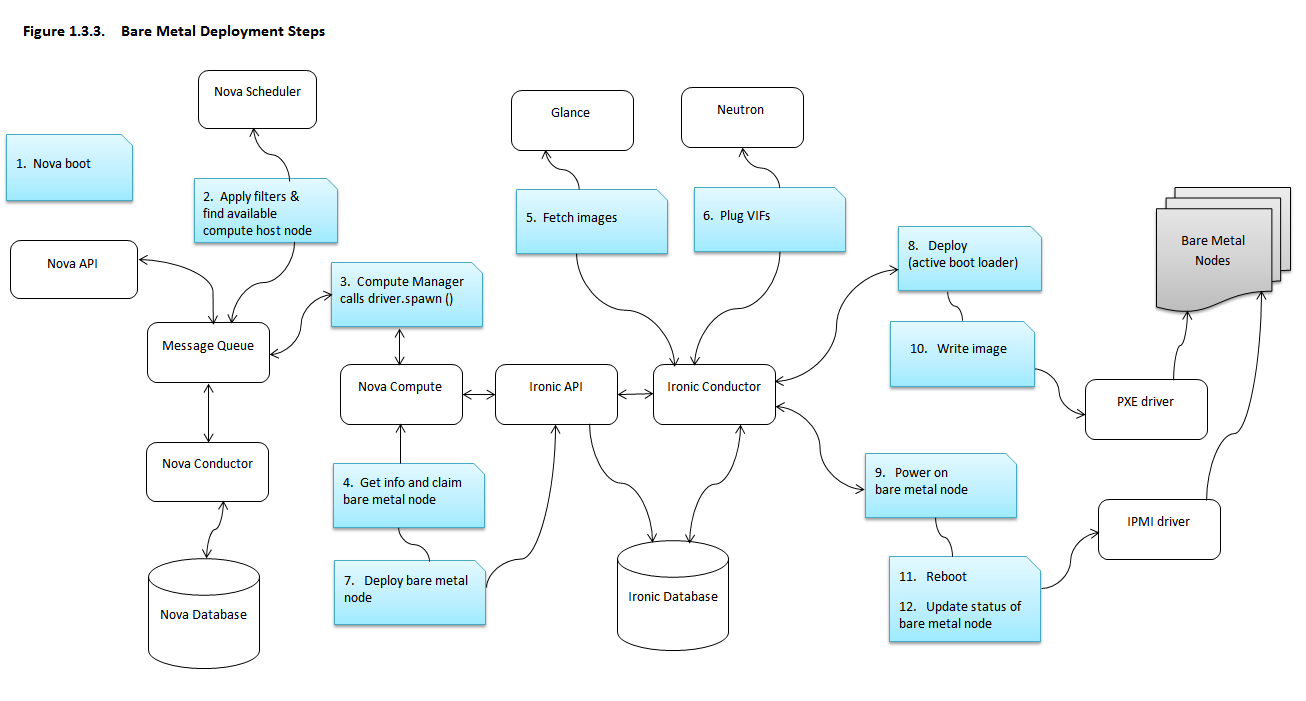
\includegraphics[scale=0.5]{deployment_steps.png}
  \caption{Ironic部署流程图\protect\footnotemark}
  \label{fig:deployment_steps}
\end{figure}
\footnotetext{来源:\url{http://docs.openstack.org/developer/ironic/_images/deployment_steps.png}}

部署关键步骤
\begin{enumerate}
  \item 根据flavor的extra\_specs中的cpu\_arch,baremetal:deploy\_kernel\_id,baremetal:deploy\_ramdisk\_id等等来搜索合适的物理主机
  \item 物理节点的信息来源于Ironic的数据库
  \item 如果Ironic使用pxe\_类的driver,则会从glance下载ramdisk和user instance images;而agent\_类的driver,则只会下载ramdisk
  \item PXE driver准备tftp的blootloader
  \item IPMI设置物理节点从pxe启动,并开机
  \item DHCP部署ramdisk。接下来,根据具体的driver,pex类的dirver通过iSCSI拷贝image到物理节点,agent\_类的driver则从tempurl下载ramdisk
  \item IPMI的驱动将重启物理服务器,完成安装
\end{enumerate}

\begin{figure}[H]
  \centering
  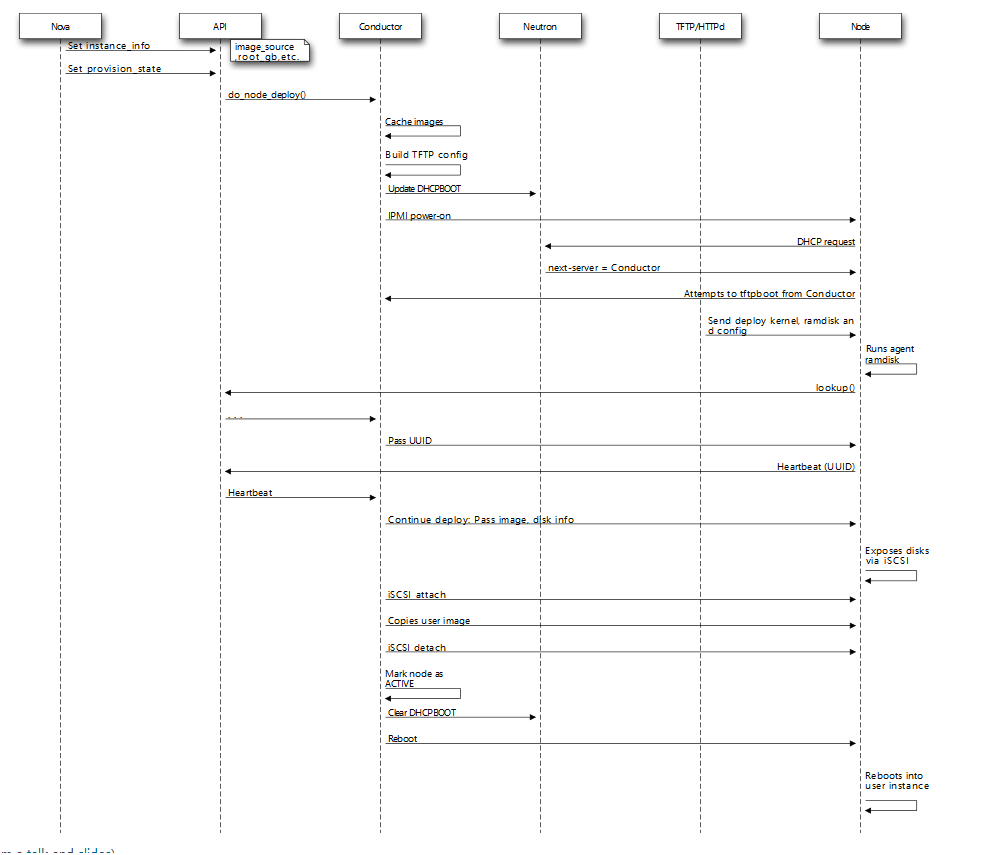
\includegraphics[scale=0.4]{boot_from_pxe.png}
  \caption{从PXE启动\protect\footnotemark}
  \label{fig:boot_from_pxe}
\end{figure}
\footnotetext{来源:\url{http://docs.openstack.org/developer/ironic/deploy/user-guide.html\#example-1-pxe-boot-and-iscsi-deploy-process}}
